\iffalse %% true for article, false for presentation
\documentclass[12pt]{article}
\usepackage{beamerarticle}
\usepackage[lmargin=1.3in,rmargin=1.3in,tmargin=0.5in,bmargin=0.5in,marginparwidth=1.5in]{geometry}
\else
\documentclass[ignorenonframetext]{beamer}
\fi
\usepackage[export]{adjustbox}
\usepackage{mathptmx}
\usepackage{natbib}
\usepackage{apalike}
\usepackage{multicol}
\usepackage{eso-pic}
\usepackage[T1]{fontenc}
\usepackage{tikz}
\usepackage[english]{babel}
\usepackage[latin1]{inputenc}
\usepackage{helvet}
\usepackage{graphicx}
\usepackage{xcolor}
\usepackage{amsmath}
\usepackage{enumitem}

\makeatletter
\gdef\SetFigFont#1#2#3#4#5{%
  \reset@font\fontsize{#1}{#2pt}%
  \fontfamily{#3}\fontseries{#4}\fontshape{#5}%
  \selectfont}%
\makeatother

\setlist[itemize]{itemsep=20pt,label=$\bullet$}

\usepackage{tikz}

\defbeamertemplate<article>{frame begin}{lined}{\par\noindent\rule{\textwidth}{1pt}\par}
\defbeamertemplate<article>{frame end}{lined}{\par\noindent\rule{\textwidth}{1pt}\par}

\newcounter{framebox}
\defbeamertemplate<article>{frame begin}{tikzed}{%
  \par\noindent\stepcounter{framebox}%
  \tikz[remember picture,overlay] %
  \path (-1ex,0) coordinate (frame top \the\value{framebox});}
\defbeamertemplate<article>{frame end}{tikzed}{%
  \hspace*{\fill}\tikz[remember picture,overlay] %
  \draw (frame top \the\value{framebox}) rectangle (1ex,0);\par}


\mode<article>
{
  \setlength{\parskip}{10pt}
  \setlength{\parindent}{0pt}

  \setbeamertemplate{frame begin}[lined]
  \setbeamertemplate{frame end}[lined]
%  \addtobeamertemplate{frame begin}{}{\setbox0=\bgroup}
%  \addtobeamertemplate{frame end}{\egroup}{}
  \usepackage{fancyhdr}
  \renewcommand{\headrulewidth}{0pt}
  \fancypagestyle{plain}{%
    \fancyhead[L]{}
    \fancyhead[C]{}
    \fancyhead[R]{}
    \fancyfoot[C]{}
    \fancyfoot[R]{\raisebox{6in}[0pt][0pt]{\hbox to 0pt{\hspace{0.3in}\framebox{\LARGE\thepage}}}}}
  \pagestyle{plain}
}

\newcommand{\cp}[1]{\textcolor{lightgray}{#1}}
\setcitestyle{authoryear,open={(},close={)}}

\mode<presentation>
{
%  \hypersetup{colorlinks=true,citecolor=green}

  \usecolortheme{default}
  \useinnertheme[shadow]{rounded}
  \useoutertheme{tsinfolines}

  \usesubitemizeitemtemplate{%
    \tiny\raise1.5pt\hbox{\color{beamerstructure}$\blacktriangleright$}%
  }
  \usesubsubitemizeitemtemplate{%
    \tiny\raise1.5pt\hbox{\color{beamerstructure}$\bigstar$}%
  }

  \setbeamersize{text margin left=1em,text margin right=1em}

% Turns off headline.
%  \setbeamertemplate{headline}[default]

  %% started as:  \usetheme[secheader]{Boadilla}
%  \usecolortheme{albatross}
  % or ...

  \setbeamercovered{invisible}
  % or whatever (possibly just delete it)

%  \addtobeamertemplate{frame title}{\begin{center}}{\end{center}}
%  Doesn't seem to do what I'd want.

}

%\beamertemplatenavigationsymbolsempty


\title{VR Graphics Programming for, well, you know}
\subtitle{Some (relatively) easy steps to virtual reality, Part 2}
\author{Tom Sgouros}
\institute{Center for Computation
    and Visualization\\Brown University\\thomas\_sgouros@brown.edu}
\date{Spring 2018}


% If you wish to uncover everything in a step-wise fashion, uncomment
% the following command:

%\beamerdefaultoverlayspecification{<+->}

\begin{document}

\maketitle

\begin{frame}
\titlepage
\end{frame}

\section{Structure of programs}

\begin{frame}{Program structure}

\begin{center}
\begin{minipage}{0.5\columnwidth}
\begin{itemize}
\item Event loop

  \begin{itemize}
  \item Event handler
  \item Animation
  \item Rendering
  \end{itemize}

\item Shaders
\end{itemize}
\end{minipage}
\end{center}
\end{frame}

\subsection{Event loop}

\begin{frame}[fragile]{Event loop}

\setlength{\fboxsep}{15pt}
\hfill Basic real-time programming structure:
\framebox{\begin{minipage}{0.25\columnwidth}

\hfill{\bfseries Initialize stuff}\hfill~

\hfill\hbox{$\downarrow$ ~~~~~~~}\hfill~

\hfill\hbox{\bfseries What changed?}\hfill~

\hfill\hbox{$\downarrow$ ~~~~~ $\uparrow$}\hfill~

\hfill\hbox{\bfseries Draw it}\hfill~
\end{minipage}}\hfill~

\begin{verbatim}
  ...
  scene.addObject(axesSet);

  scene.setLookAtPosition(glm::vec3(0.0f, 0.0f, 0.0f));
  scene.setCameraPosition(glm::vec3(1.0f, 2.0f, 7.5f));
  scene.prepare();

  glutMainLoop();
  return(0);
\end{verbatim}
\end{frame}


\subsection{Event handler}

\begin{frame}{Different kinds of input}

\begin{center}
\begin{minipage}{0.75\columnwidth}\raggedright
\begin{description}

\item[Synchronous:] On {\color{red}my} schedule.\\
  Prompt for input and, um, prompt for input.  Also sometimes polled input.


\vspace{20pt}

\item[Asynchronous:] On {\color{red}your} schedule.\\
  Mouse movements, head movements, wand movements,
  button presses, typing, gesture recognition\ldots

\vspace{10pt}
~~~a/k/a \emph{events}, \emph{interrupts}.

\end{description}
\end{minipage}
\end{center}

\end{frame}


\begin{frame}[fragile]{Event handler}

Handles asynchronous input.

\begin{verbatim}
void processNormalKeys(unsigned char key, int x, int y) {

  float step = 0.5f;

  switch (key) {
  case 27:    exit(0);
  case 'a':
    scene.addToCameraPosition(glm::vec3(-step, 0.0f, 0.0f));
    break;
  case 'q':
    scene.addToCameraPosition(glm::vec3( step, 0.0f, 0.0f));
    break;
  case 's':
    ...
\end{verbatim}
\end{frame}


\section{Animation}

\begin{frame}{Animation}

\begin{center}
\begin{minipage}{0.75\columnwidth}\raggedright
\begin{description}

\item[Change what is seen] ~~\\
  Motion in space, motion within scene component, model changing shape


\vspace{20pt}

\item[Change how it is seen] ~\\
  Camera motion, lighting change

\end{description}
\end{minipage}
\end{center}

\end{frame}




\begin{frame}[fragile]{Render function}

Combines animation and drawing stuff.

\begin{verbatim}

void renderScene() {
  ...
  glm::vec3 pos = tetrahedron->getPosition();
  oscillator += oscillationStep;
  pos.x = sin(oscillator);
  pos.y = 1.0f - cos(oscillator);
  tetrahedron->setPosition(pos);

  glClear(GL_COLOR_BUFFER_BIT | GL_DEPTH_BUFFER_BIT);
  scene.load();
  scene.draw(scene.getViewMatrix(), scene.getProjMatrix());

  glutSwapBuffers();
\end{verbatim}
\end{frame}


\subsection{Shaders}

\begin{frame}[fragile]{Shaders}
OpenGL innovation, historically related to the transformation of
graphics cards to GPUs.  Looks C-ish.  Biggest problem is the lack of
clarity about inputs and outputs.

\begin{verbatim}
#version 120

uniform mat4 projMatrix, viewMatrix, modelMatrix;
attribute vec4 position, color;
varying vec4 colorFrag;

void main()
{
  colorFrag = color;
  gl_Position = projMatrix * viewMatrix * modelMatrix * position ;
}
\end{verbatim}
\end{frame}

\begin{frame}[fragile]{Shaders}
OpenGL innovation, historically related to the transformation of
graphics cards to GPUs.  Looks C-ish.  Biggest problem is the lack of
clarity about inputs and outputs.  Slightly improved in OpenGL 3.

\begin{verbatim}
#version 330

uniform mat4 projMatrix, viewMatrix, modelMatrix;
layout(location=0) in vec4 position;
layout(location=1) in vec4 color;
out vec4 colorFrag;

void main()
{
  colorFrag = color;
  gl_Position = projMatrix * viewMatrix * modelMatrix * position ;
}
\end{verbatim}
\end{frame}

\begin{frame}[fragile]{Prepare a shader}

A shader has to be given an ID, compiled and then a ``program'' is
created and the shader(s) are linked to it.  Here's the vertex shader.
The other shaders would be virtually the same.

\begin{verbatim}
shaderMgr::compileShaders() {...
  shaderID = glCreateShader(GL_VERTEX_SHADER);
  const char* vs = shaderText.c_str();
  glShaderSource(shaderID, 1, &vs, NULL);
  glCompileShader(shaderID);
  errorLog = _getShaderInfoLog(shaderID);
  if (errorLog.size() > 1)
    std::cerr << "** Vertex compile error in " ...;
  programID = glCreateProgram();
  glAttachShader(programID, shaderID);
  glLinkProgram(programID);
  ...
\end{verbatim}
\end{frame}


\begin{frame}[fragile]{Shader input}

Then you have to make a buffer in your program correspond to an attribute name in
the shader.

\begin{verbatim}
  glUseProgram(programID);
  attribID = glGetAttribLocation(programID, attribName.c_str());
\end{verbatim}

\begin{verbatim}
  glGenBuffers(1, &attribBufferID);
\end{verbatim}


\begin{verbatim}
  glEnableVertexAttribArray(attribID);
  glBindBuffer(GL_ARRAY_BUFFER, attribBufferID);
  glBufferData(GL_ARRAY_BUFFER, attribLengthInBytes, attrib[0],
               GL_STATIC_DRAW);


\end{verbatim}
\end{frame}

\begin{frame}[fragile]{More shader input}

Then you have to make a buffer in your program correspond to a uniform
name in the shader.

\begin{verbatim}
  glUseProgram(programID);
  unifID = glGetUniformLocation(programID, unifName.c_str());
\end{verbatim}


\begin{verbatim}
  glUniformMatrix4fv(unifID, 1, false, &unifMatrix[0][0]);
\end{verbatim}
\end{frame}

\begin{frame}[fragile]{Draw it!}

Bind the buffer, say what's in it, draw it.

\begin{verbatim}

  glBindBuffer(GL_ARRAY_BUFFER, verticesBufferID);
  glVertexAttribPointer(verticesID, verticesComponentsPerVertex,
                        GL_FLOAT, 0, 0, 0);

  glBindBuffer(GL_ARRAY_BUFFER, colorsBufferID);
  glVertexAttribPointer(colorsID, colorsComponentsPerVertex,
                        GL_FLOAT, 0, 0, 0);

  glDrawArrays(drawType, 0, verticesCount);
\end{verbatim}
\end{frame}

\begin{frame}[fragile]{Draw with more complicated buffers}
Buffers can also have interleaved data.

\begin{verbatim}
  glBindBuffer(GL_ARRAY_BUFFER, interleavedBufferID);

  glVertexAttribPointer(verticesID, 3,
                        GL_FLOAT, GL_FALSE, stride,
                        BUFFER_OFFSET(0));
  glVertexAttribPointer(colorsID, 3,
                        GL_FLOAT, GL_FALSE, stride,
                        BUFFER_OFFSET(3));
  glDrawArrays(drawType, 0, verticesCount);
\end{verbatim}
\end{frame}

\begin{frame}[fragile]{Using BSG, step 1}
Deal with shaders

\begin{verbatim}
  bsg::bsgPtr<bsg::lightList> lights = new bsg::lightList();
  lights->addLight(glm::vec4(0.0f, 0.0f, 3.0f, 1.0f));

  bsg::bsgPtr<bsg::shaderMgr> shader = new bsg::shaderMgr();
  shader->addLights(lights);
  shader->addShader(bsg::GLSHADER_VERTEX, vertexFile);
  shader->addShader(bsg::GLSHADER_FRAGMENT, fragmentFile);
  shader->compileShaders();

  bsg::bsgPtr<bsg::textureMgr> texture = new bsg::textureMgr();
  texture->readFile(bsg::texturePNG, "../data/gladiolas-sq.png");
  shader->addTexture(texture);
\end{verbatim}
\end{frame}

\begin{frame}[fragile]{Using BSG, step 2}
Deal with objects, build the scene.

\begin{verbatim}
  bsg::drawableRectangle* bigRectangle, smallRectangle;
  bsg::drawableCollection* rectGroup;

  bigRectangle = new bsg::drawableRectangle(shader, 9.0f, 9.0f, 4);
  smallRectangle = new bsg::drawableRectangle(shader, 3.0f, 5.0f, 2);

  smallRectangle->setPosition(1.0f, 1.0f, 0.5f);

  rectGroup = new bsg::drawableCollection("rectangles");

  rectGroup->addObject("big", bigRectangle);
  rectGroup->addObject("small", smallRectangle);

  scene.addObject(rectGroup);

\end{verbatim}
\end{frame}

\begin{frame}[fragile]{Using BSG, step 3}
Finish up.

\begin{verbatim}
  axes = new bsg::drawableAxes(axesShader, 100.0f);
  scene.addObject(axes);

  scene.setLookAtPosition(glm::vec3(0.0f, 0.0f, 0.0f));
  scene.setCameraPosition(glm::vec3(1.0f, 2.0f, 7.5f));

  scene.prepare();

  glutMainLoop();
\end{verbatim}
\end{frame}


\begin{frame}{Admire the result}

Sigh with relief.
\begin{center}
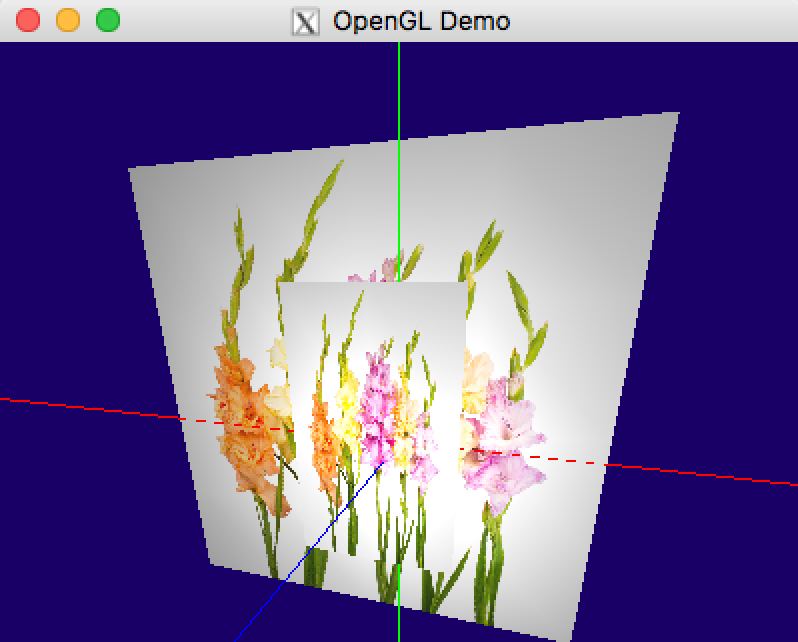
\includegraphics[width=0.6\columnwidth]{images/treeDemo2.png}
\end{center}

\end{frame}


\end{document}
